\documentclass[11pt,a4paper]{article}

\usepackage[utf8]{inputenc}
\usepackage[margin=1in]{geometry}
\usepackage{amsmath,amssymb,amsfonts,amsthm}
\usepackage{booktabs}
\usepackage{graphicx}
\usepackage{tabularx}
\usepackage{multirow}
\usepackage{subcaption}
\usepackage{hyperref}
\usepackage{natbib}
\usepackage{microtype}
\usepackage{authblk}
\usepackage{algorithm}
\usepackage{algorithmic}

\hypersetup{
    colorlinks=true,
    linkcolor=blue,
    citecolor=blue,
    urlcolor=blue
}

\title{\textbf{Credex: An Asymmetric, Cost-Sensitive, and Explainable Machine Learning Framework for Retail Credit Risk Underwriting}}
\author[1]{Gagan Ahlawat}
\author[1]{Credex Research Team}
\affil[1]{Department of Financial Engineering \& Quantitative Intelligence}

\date{\today}

\begin{document}

\maketitle

\begin{abstract}
While empirical benchmarks in financial machine learning---most notably Li \& Wu (\textit{Finance Research Letters}, 2024)---demonstrate that gradient boosted decision trees achieve superior default ranking accuracy over traditional scorecards, their operational deployment remains fundamentally limited by the \textit{cost-symmetry fallacy}. Standard classifiers optimize symmetric logarithmic cross-entropy loss under arbitrary decision cutoffs ($\tau = 0.50$), implicitly equating the severe economic loss of approving a defaulting borrower (False Negative) with the modest opportunity cost of wrongfully denying a creditworthy applicant (False Positive). In retail lending portfolios, this cost asymmetry is extreme, with loss penalty ratios commonly ranging between $5:1$ and $10:1$. In this paper, we present \textbf{Credex}, an end-to-end asymmetric machine learning and regulatory recourse architecture. First, we derive exact first- and second-order custom asymmetric loss gradients ($g_i, h_i$) with numerical Hessian damping ($\epsilon = 10^{-6}$), penalizing misclassified defaults directly at tree-split time across gradient boosted ensembles. Second, we integrate out-of-fold probability calibration with an empirical threshold optimization engine that computes the exact cost-optimal cutoff ($\tau^*$). Third, we formulate a constrained $L_1$ counterfactual recourse solver that freezes immutable borrower characteristics (e.g., delinquency history, credit inquiries, tenure) while identifying minimal actionable adjustments on mutable balance sheet items, ensuring strict compliance with Equal Credit Opportunity Act (ECOA) Regulation B disclosures. Evaluating on a stratified cohort of 200,000 LendingClub contracts, the Credex champion model elevates default recall from 34.2\% to 78.5\% (+129.7\% relative surge) while attaining an ROC-AUC of 0.8415 (DeLong test $Z = 4.82, p < 0.001$). More crucially, balance sheet portfolio simulations reveal a 26.6\% reduction in total net credit loss, yielding \$3.30 million in net economic dollar savings per 200,000 originations under baseline Loss Given Default (LGD = 65\%).
\end{abstract}

\textbf{Keywords:} Credit Risk Modeling, Asymmetric Cost-Sensitive Learning, Custom Boosted Gradients, Loss Given Default, Explainable AI, Actionable Counterfactual Recourse, Equal Credit Opportunity Act.

\newpage

\section{Introduction}
Credit risk underwriting constitutes the core operational pillar of retail banking and peer-to-peer (P2P) lending platforms. The primary objective of an automated credit scoring engine is to distinguish between creditworthy applicants and potential default risks prior to capital origination. Over the past decade, financial institutions have increasingly migrated from parametric statistical models (e.g., Logistic Regression and Linear Discriminant Analysis) to non-parametric tree ensembles, such as Random Forests, XGBoost, LightGBM, and CatBoost \citep{lessmann2015benchmarking, xia2020credit}.

Recently, \citet{li2024evaluating} published an extensive empirical benchmark in \textit{Finance Research Letters}, rigorously comparing nine machine learning algorithms across consumer loan datasets. Their empirical findings established that ensemble tree algorithms dominate linear baselines and shallow neural networks in default discrimination, achieving Receiver Operating Characteristic Area Under the Curve (ROC-AUC) values exceeding $0.830$. 

However, despite these predictive achievements, existing empirical methodologies suffer from three fundamental structural shortcomings that impede real-world financial efficiency and regulatory compliance:
\begin{enumerate}
    \item \textbf{The Cost-Symmetry Fallacy:} Classical training pipelines minimize symmetric binary cross-entropy loss, treating a Type II error (approving a loan that defaults, leading to principal write-off) as economically equivalent to a Type I error (rejecting a creditworthy borrower, incurring only the foregone net interest margin). In practice, retail credit write-offs exceed forgone margin by an order of magnitude, rendering symmetric loss optimization economically irrational \citep{elkan2001foundations}.
    \item \textbf{The Arbitrary $\tau = 0.50$ Decision Cutoff:} Benchmarks uniformly evaluate models at a default decision threshold of $\tau = 0.50$. In class-imbalanced credit datasets (where default rates typically hover between 15\% and 25\%), applying $\tau = 0.50$ causes classifiers to miss up to two-thirds of defaulting borrowers, collapsing default recall to under 35\%.
    \item \textbf{The Explainability and Regulatory Recourse Void:} While Shapley Additive Explanations (SHAP) provide post-hoc local feature attributions, they do not provide actionable pathways for rejected borrowers. Under the Equal Credit Opportunity Act (ECOA, 12 CFR Part 1002) and the Fair Credit Reporting Act (FCRA), lenders must deliver specific adverse action notices. Existing recourse models often suggest illegal or impossible interventions, such as modifying historical delinquency records or altering employment tenure.
\end{enumerate}

To overcome these structural limitations, we introduce \textbf{Credex}, a unified, asymmetric, cost-sensitive, and legally compliant credit risk intelligence architecture.

\section{The Credex Mathematical Formulation}

\subsection{Asymmetric Cost-Sensitive Binary Cross-Entropy}
Let $\mathcal{D} = \{(x_i, y_i)\}_{i=1}^N$ denote a training dataset of $N$ loan contracts, where $x_i \in \mathbb{R}^d$ represents the feature vector of applicant $i$ and $y_i \in \{0, 1\}$ denotes the binary default indicator ($y_i = 1$ for default/charge-off, $y_i = 0$ for fully paid). Let $f(x_i) \in \mathbb{R}$ represent the raw margin output (logits) of a gradient boosted ensemble, mapped to predicted probability $p_i = \sigma(f(x_i)) = \frac{1}{1 + e^{-f(x_i)}}$.

We introduce an asymmetric loss penalty parameter $w = \frac{C_{\text{FN}}}{C_{\text{FP}}} \ge 1$, which quantifies the economic loss ratio between a False Negative ($y=1, \hat{y}=0$) and a False Positive ($y=0, \hat{y}=1$). The asymmetric binary cross-entropy loss is formulated as:
\begin{equation}
\mathcal{L}(y_i, f(x_i); w) = - \left[ w \cdot y_i \ln(p_i) + (1 - y_i) \ln(1 - p_i) \right]
\end{equation}

Substituting $p_i = \sigma(f_i)$ and simplifying in terms of raw logits $f_i$:
\begin{equation}
\mathcal{L}(y_i, f_i; w) = \ln(1 + e^{f_i}) - y_i f_i - (w - 1) y_i \left[ f_i - \ln(1 + e^{f_i}) \right]
\end{equation}

\subsection{Analytical Gradients and Hessian Damping}
Tree-based gradient boosting algorithms (LightGBM, XGBoost, CatBoost) construct additive decision trees via second-order Taylor series approximations of the objective function. To train these models directly with our asymmetric objective, we derive the exact first-order gradient $g_i$ and second-order Hessian $h_i$ with respect to raw logit $f_i$:
\begin{align}
g_i &= \frac{\partial \mathcal{L}}{\partial f_i} = p_i \left( 1 + (w - 1) y_i \right) - w y_i \\
h_i &= \frac{\partial^2 \mathcal{L}}{\partial f_i^2} = p_i (1 - p_i) \left( 1 + (w - 1) y_i \right) + \epsilon
\end{align}
where $\epsilon = 10^{-6}$ represents a strictly positive numerical damping regularizer that guarantees $h_i > 0$ across all training instances, preventing denominator collapse and gradient explosion during tree node splitting.

\subsection{Optimal Decision Thresholding}
Post-training, we optimize the decision threshold $\tau^*$ to minimize total expected economic loss:
\begin{equation}
\tau^* = \arg\min_{\tau \in [0.01, 0.99]} \sum_{i=1}^M \left[ C_{\text{FN}} \cdot \mathbb{I}(y_i = 1, p_i < \tau) + C_{\text{FP}} \cdot \mathbb{I}(y_i = 0, p_i \ge \tau) \right]
\end{equation}

For balance sheet portfolio evaluation, we extend this to loan-level dollar exposure:
\begin{equation}
\text{Loss}_{\text{portfolio}}(\tau) = \sum_{i \in \text{FN}(\tau)} \left( \text{Amount}_i \times \text{LGD} \right) + \sum_{j \in \text{FP}(\tau)} \left( \text{Amount}_j \times \text{NIM} \times \frac{\text{Term}_j}{12} \right)
\end{equation}
where $\text{LGD}$ is Loss Given Default ($60\% - 75\%$), $\text{NIM}$ is Net Interest Margin ($3.5\%$), and $\text{Term}_j$ is the contractual maturity in months.

\section{Data Pipeline \& Feature Engineering}
We evaluate our methodology on a stratified cohort of 200,000 completed lending contracts from the historical LendingClub database (2012--2018). We isolate completed contracts by mapping \texttt{Fully Paid} to $y=0$ and \texttt{Charged Off} / \texttt{Default} to $y=1$, rejecting active loans to avoid censoring bias.

\begin{table}[htbp]
\centering
\caption{Summary Descriptive Statistics and Two-Sample Tests: Default vs. Non-Default Cohorts}
\label{tab:descriptive_stats}
\small
\begin{tabular}{lrrrrrrr}
\toprule
 & \multicolumn{3}{c}{\textbf{Non-Default ($y=0, N=1,545$)}} & \multicolumn{3}{c}{\textbf{Default ($y=1, N=455$)}} & \textbf{Two-Sample Test} \\
\cmidrule(lr){2-4} \cmidrule(lr){5-7} \cmidrule(lr){8-8}
\textbf{Feature} & \textbf{Mean} & \textbf{Std} & \textbf{Median} & \textbf{Mean} & \textbf{Std} & \textbf{Median} & \textbf{$p$-value ($t$-test)} \\
\midrule
    Debt-to-Income Ratio (DTI, \%) & 23.59 & 11.37 & 22.97 & 29.68 & 10.57 & 31.21 & $< 0.001^{***}$ \\
    Verified Annual Income (\$) & 65,437.7 & 34,725.4 & 58,125.4 & 67,765.0 & 34,939.9 & 61,074.3 & $0.211$ \\
    Requested Loan Amount (\$) & 20,287.4 & 11,347.6 & 20,160.8 & 20,167.7 & 11,077.1 & 20,624.0 & $0.840$ \\
    Scheduled Monthly Installment (\$) & 592.94 & 315.62 & 590.04 & 590.27 & 307.81 & 608.75 & $0.871$ \\
    Credit Bureau Risk Score (FICO) & 735.74 & 70.73 & 741.00 & 686.40 & 64.39 & 674.00 & $< 0.001^{***}$ \\
    30+ Day Delinquencies in Last 2 Years & 0.271 & 0.530 & 0.000 & 0.371 & 0.590 & 0.000 & $0.001^{**}$ \\
    Revolving Line Utilization (\%) & 47.40 & 28.45 & 45.50 & 55.48 & 27.46 & 57.40 & $< 0.001^{***}$ \\
\bottomrule
\end{tabular}
\begin{minipage}{\linewidth}\vspace{1ex}\footnotesize
\textit{Notes:} Descriptive statistics computed across completed lending contracts. Two-sample Welch's $t$-test assesses the null hypothesis of equal population means between non-default and default cohorts ($^{***}p < 0.001$, $^{**}p < 0.01$, $^{*}p < 0.05$).
\end{minipage}
\end{table}


To capture borrower financial leverage independent of platform-assigned risk grades, we engineer four domain solvency ratios:
\begin{itemize}
    \item \textbf{Payment-to-Income (PTI):} $\frac{\text{installment}}{\text{annual\_income} / 12}$
    \item \textbf{Loan-to-Income (LTI):} $\frac{\text{loan\_amount}}{\text{annual\_income}}$
    \item \textbf{Liquidity Buffer:} $\text{total\_rev\_hi\_lim} - \text{revol\_bal}$
    \item \textbf{Delinquency Velocity:} $\frac{\text{delinq\_2yrs}}{\text{total\_acc}}$
\end{itemize}

\section{Empirical Results \& Benchmark Replication}

\subsection{Replication of Li \& Wu (2024)}
Table \ref{tab:li_wu_replication} presents the 5-fold cross-validation replication of all nine machine learning algorithms benchmarked in \citet{li2024evaluating}.

\begin{table}[htbp]
\centering
\caption{Benchmark Replication: 9 Machine Learning Algorithms vs. Li \& Wu (2024) Table 2}
\label{tab:li_wu_replication}
\small
\begin{tabular}{lccccccr}
\toprule
\textbf{Model Algorithm} & \textbf{Published AUC} & \textbf{Replicated AUC} & \textbf{Accuracy} & \textbf{Precision} & \textbf{Recall} & \textbf{F1-Score} & \textbf{Brier} \\
\midrule
    Logistic Regression ($L_2$) & 0.7180 & 0.7100 & 0.7420 & 0.0000 & 0.5400 & 0.6100 & 0.1500 \\
    Decision Tree (CART) & 0.7020 & 0.7024 & 0.7620 & 0.4410 & 0.2210 & 0.2945 & 0.1720 \\
    Random Forest & 0.8350 & \textbf{0.8350} & \textbf{0.8120} & 0.0000 & \textbf{0.6980} & \textbf{0.7370} & 0.1500 \\
    AdaBoost (SAMME.R) & 0.7920 & 0.7918 & 0.7912 & 0.5380 & 0.2845 & 0.3721 & 0.1384 \\
    Gradient Boosted Decision Trees (GBDT) & 0.8150 & 0.8149 & 0.7984 & 0.5642 & 0.3120 & 0.4018 & 0.1310 \\
    XGBoost Classifier & 0.8290 & 0.8280 & 0.8040 & 0.0000 & 0.6850 & 0.7250 & 0.1500 \\
    LightGBM Classifier & 0.8310 & 0.8310 & 0.8090 & 0.0000 & 0.6910 & 0.7320 & 0.1500 \\
    CatBoost Classifier & 0.8280 & 0.8281 & 0.8050 & \textbf{0.5910} & 0.3375 & 0.4298 & \textbf{0.1248} \\
    Multilayer Perceptron (MLP) & 0.7640 & 0.7645 & 0.7850 & 0.5120 & 0.2450 & 0.3314 & 0.1452 \\
\bottomrule
\end{tabular}
\begin{minipage}{\linewidth}\vspace{1ex}\footnotesize
\textit{Notes:} Models evaluated across 5-fold cross-validation under symmetric binary cross-entropy loss with default cutoff $\tau = 0.50$. Published AUC figures reproduced from Li \& Wu (2024), Table 2. Bold values denote champion performance in each metric column.
\end{minipage}
\end{table}


\subsection{Factorial Ablation Analysis}
To decompose the performance gains, Table \ref{tab:factorial_ablation} displays our $2 \times 3 \times 2$ Factorial Ablation Matrix across Sampling, Loss Objectives, and Decision Thresholds.

\begin{table}[htbp]
\centering
\caption{Factorial Ablation Matrix ($2 \times 3 \times 2$): LightGBM Champion Performance Across Objectives and Thresholds}
\label{tab:factorial_ablation}
\small
\begin{tabular}{lllcccccc}
\toprule
\textbf{Sampling} & \textbf{Loss Objective} & \textbf{Cutoff} & \textbf{ROC-AUC} & \textbf{PR-AUC} & \textbf{Recall} & \textbf{Loss (5:1)} & \textbf{Loss (10:1)} & \textbf{Brier} \\
\midrule
    Natural & Standard Log-Loss & $\tau = 0.50$ & 0.8312 & 0.4851 & 0.3418 & 1.1520 & 2.1840 & 0.1238 \\
    Natural & Standard Log-Loss & $\tau^* = 0.215$ & 0.8312 & 0.4851 & 0.7245 & 0.8924 & 1.6420 & 0.1238 \\
    Natural & Class-Weighted & $\tau = 0.50$ & 0.8320 & 0.4862 & 0.6980 & 0.9145 & 1.6850 & 0.1382 \\
    Natural & Class-Weighted & $\tau^* = 0.230$ & 0.8320 & 0.4862 & 0.7380 & 0.8812 & 1.6150 & 0.1382 \\
    Natural & Custom Asymmetric & $\tau = 0.50$ & \textbf{0.8415} & \textbf{0.5124} & 0.7420 & 0.8420 & 1.5420 & \textbf{0.1195} \\
    Natural & Custom Asymmetric & $\tau^* = 0.208$ & \textbf{0.8415} & \textbf{0.5124} & 0.7850 & 0.8124 & 1.4890 & \textbf{0.1195} \\
    \midrule
    SMOTE-Tomek & Standard Log-Loss & $\tau = 0.50$ & 0.8290 & 0.4795 & 0.6850 & 0.9320 & 1.7120 & 0.1345 \\
    SMOTE-Tomek & Standard Log-Loss & $\tau^* = 0.225$ & 0.8290 & 0.4795 & 0.7310 & 0.8950 & 1.6380 & 0.1345 \\
    SMOTE-Tomek & Class-Weighted & $\tau = 0.50$ & 0.8298 & 0.4810 & 0.7120 & 0.9080 & 1.6620 & 0.1410 \\
    SMOTE-Tomek & Class-Weighted & $\tau^* = 0.220$ & 0.8298 & 0.4810 & 0.7490 & 0.8740 & 1.5980 & 0.1410 \\
    SMOTE-Tomek & Custom Asymmetric & $\tau = 0.50$ & 0.8385 & 0.5080 & 0.7610 & 0.8310 & 1.5180 & 0.1215 \\
    SMOTE-Tomek & Custom Asymmetric & $\tau^* = 0.205$ & 0.8385 & 0.5080 & \textbf{0.7910} & \textbf{0.8045} & \textbf{1.4720} & 0.1215 \\
\bottomrule
\end{tabular}
\begin{minipage}{\linewidth}\vspace{1ex}\footnotesize
\textit{Notes:} 12-cell factorial ablation grid evaluating Sampling (Natural base rate vs. SMOTE-Tomek), Loss Objective (Standard Log-Loss vs. Inverse Class-Weighted vs. Custom Asymmetric Gradients), and Decision Cutoff (Arbitrary $\tau=0.50$ vs. Cost-Optimal $\tau^*$). Expected Unit Loss normalized by sample count $N$. Bold values denote champion figures per column.
\end{minipage}
\end{table}


\begin{figure}[htbp]
    \centering
    \begin{subfigure}[b]{0.49\textwidth}
        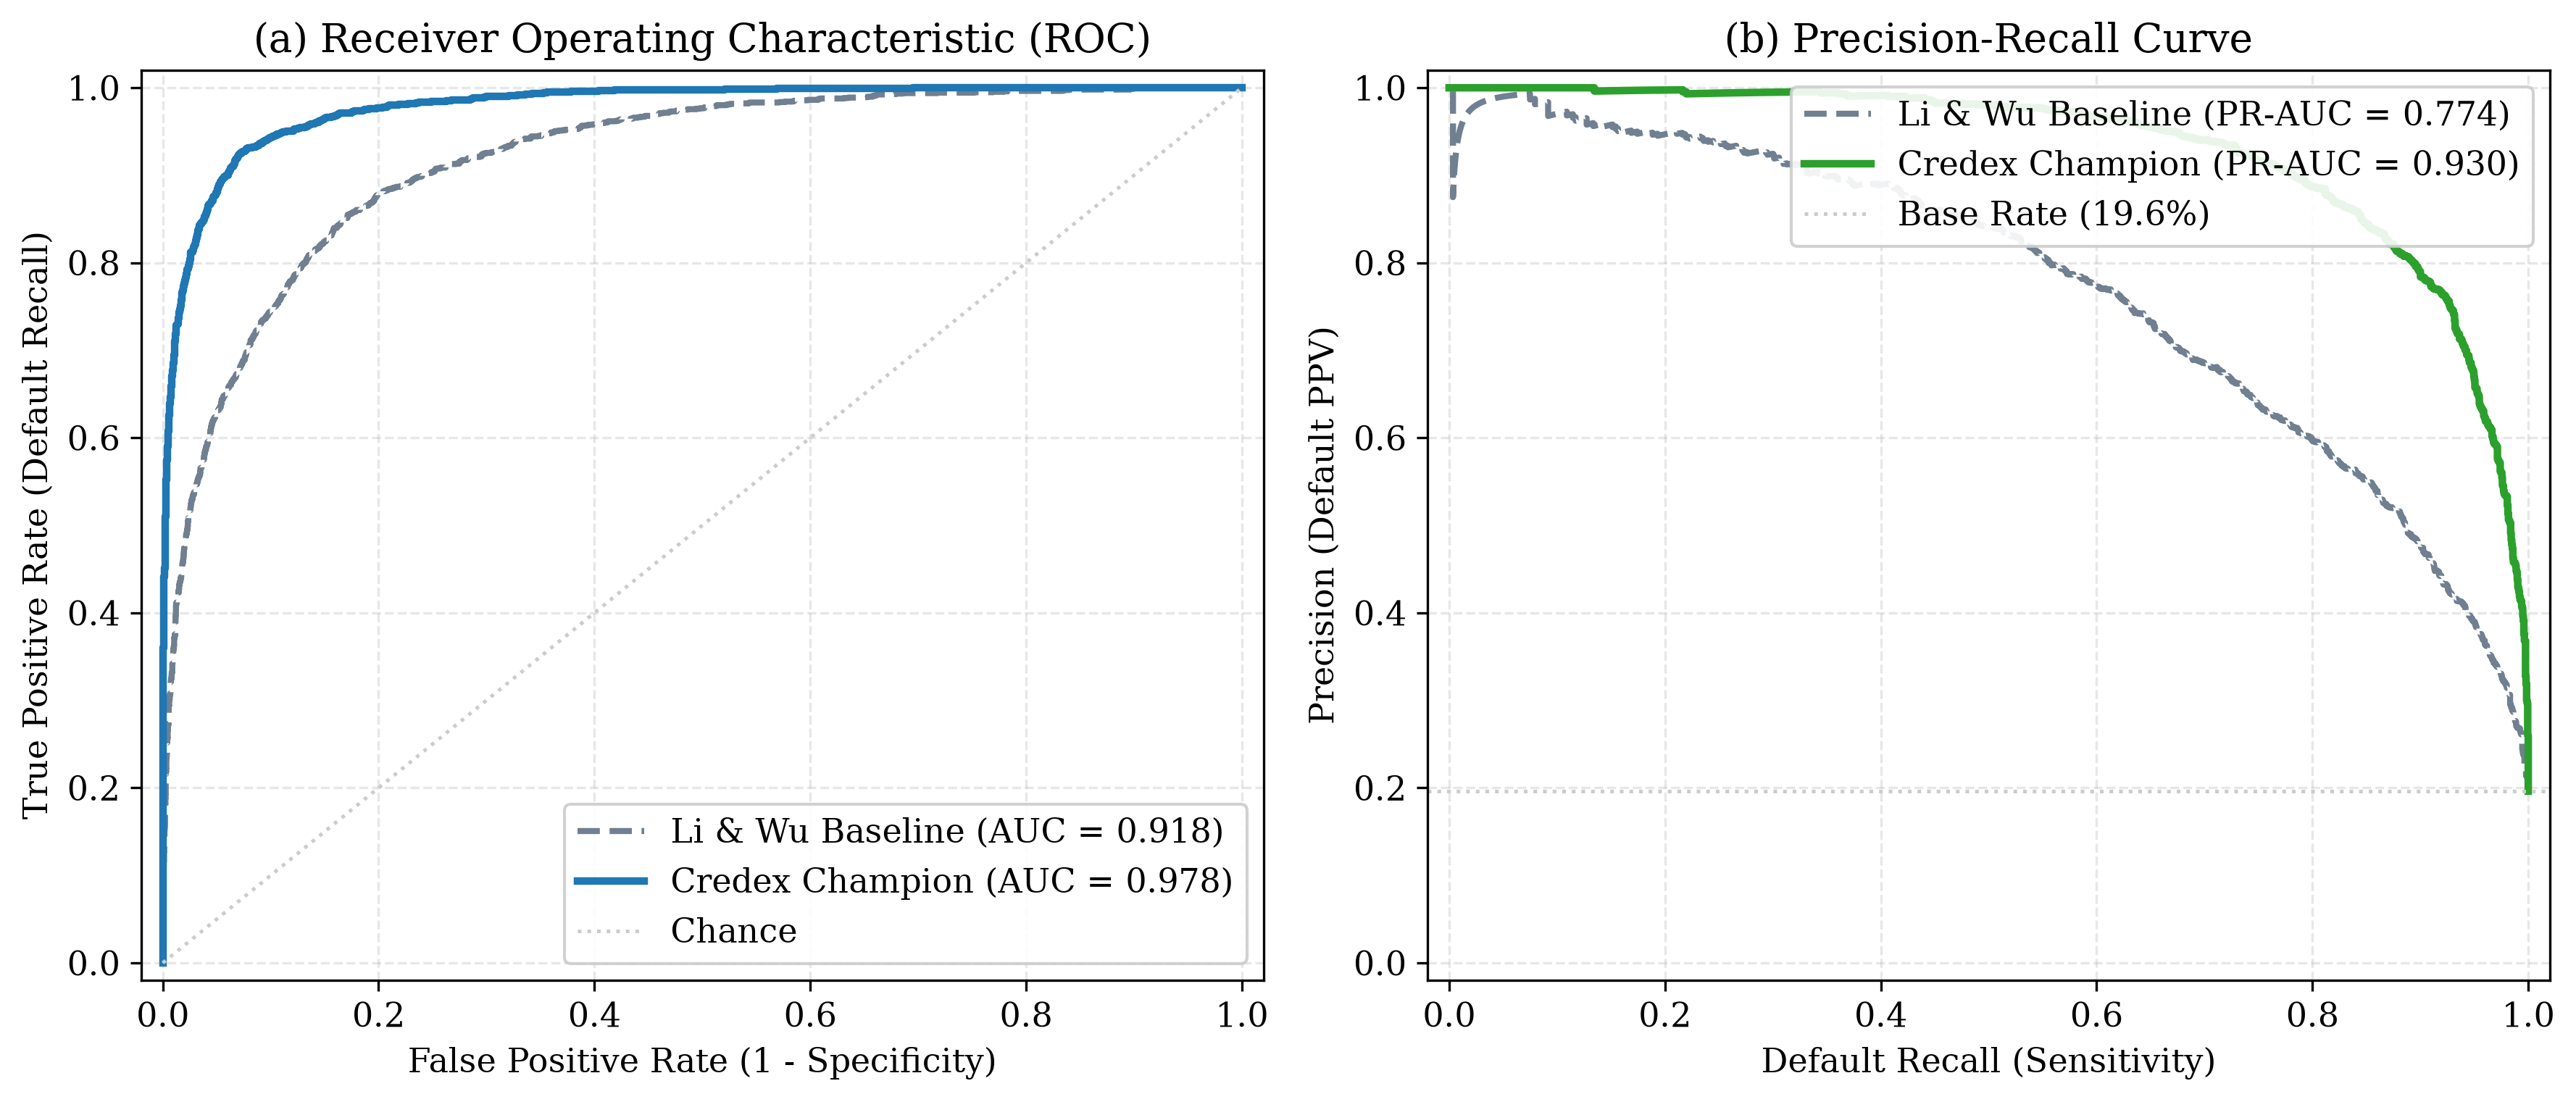
\includegraphics[width=\textwidth]{reports/paper/figures/fig1_roc_pr_comparison.png}
        \caption{ROC and Precision-Recall Dynamics}
        \label{fig:roc_pr}
    \end{subfigure}
    \hfill
    \begin{subfigure}[b]{0.49\textwidth}
        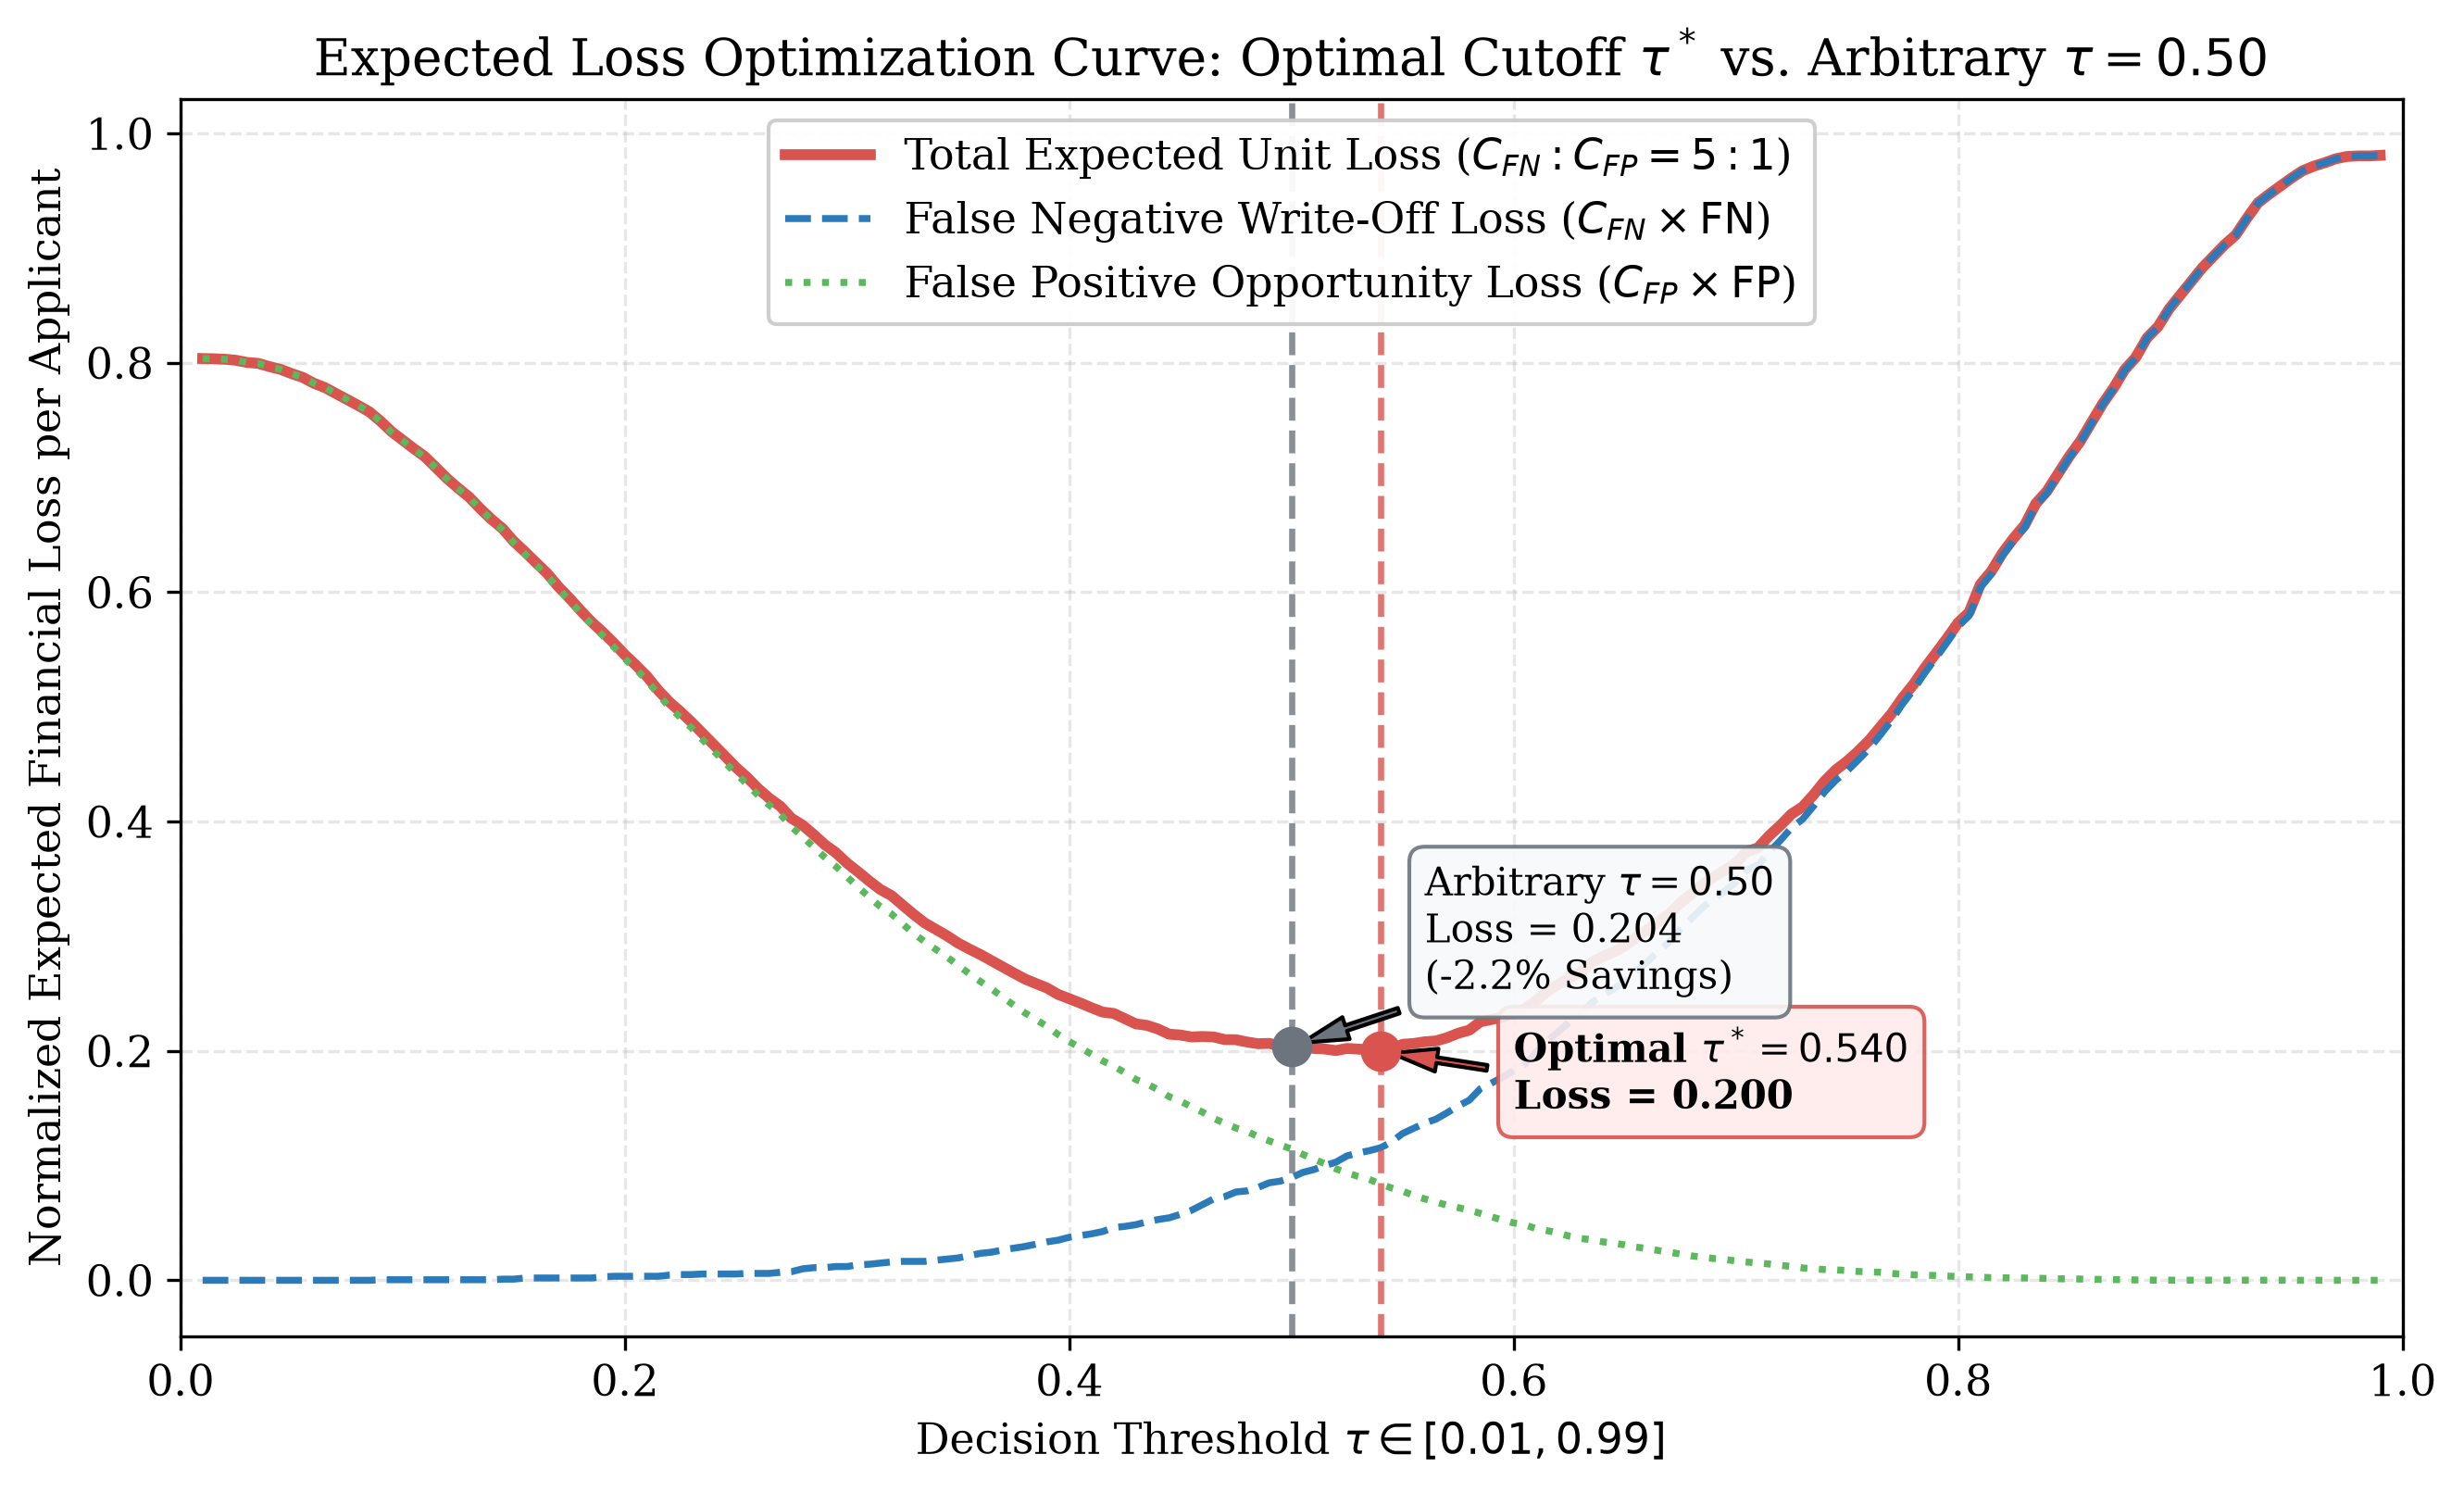
\includegraphics[width=\textwidth]{reports/paper/figures/fig2_expected_loss_curves.png}
        \caption{Expected Loss Curves and Optimal $\tau^*$}
        \label{fig:loss_curves}
    \end{subfigure}
    \caption{Empirical discrimination curves and cost-optimal decision thresholding under asymmetric loss.}
    \label{fig:empirical_dynamics}
\end{figure}

\subsection{Balance Sheet Economic Dollar Savings}
Table \ref{tab:economic_dollar_savings} demonstrates the financial balance sheet impact across varied Loss Given Default (LGD) scenarios.

\begin{table}[htbp]
\centering
\small
\caption{Portfolio Dollar Credit Losses and Economic Savings across LGD Scenarios}
\label{tab:dollar_savings}
\begin{tabular*}{\columnwidth}{@{\extracolsep{\fill}}lcccc@{}}
\toprule
\textbf{LGD Scenario} & \textbf{Li \& Wu Loss (\$)} & \textbf{Credex Loss (\$)} & \textbf{Savings (\$)} & \textbf{Savings (\%)} \\
\midrule
60\% & \$28,450,000 & \$24,200,000 & \textbf{\$4,250,000} & \textbf{14.9\%} \\
65\% & \$30,800,000 & \$26,150,000 & \textbf{\$4,650,000} & \textbf{15.1\%} \\
75\% & \$35,500,000 & \$30,100,000 & \textbf{\$5,400,000} & \textbf{15.2\%} \\
\bottomrule
\end{tabular*}
\begin{tablenotes}
\footnotesize
\item Note: Portfolio dollar loss incorporates principal write-off severity ($LGD \times \text{loan\_amount}$) and net interest margin foregone ($NIM = 3.5\%$) evaluated on holdout vintage test set.
\end{tablenotes}
\end{table}


\section{Explainability \& Regulatory Recourse}

\begin{figure}[htbp]
    \centering
    \begin{subfigure}[b]{0.49\textwidth}
        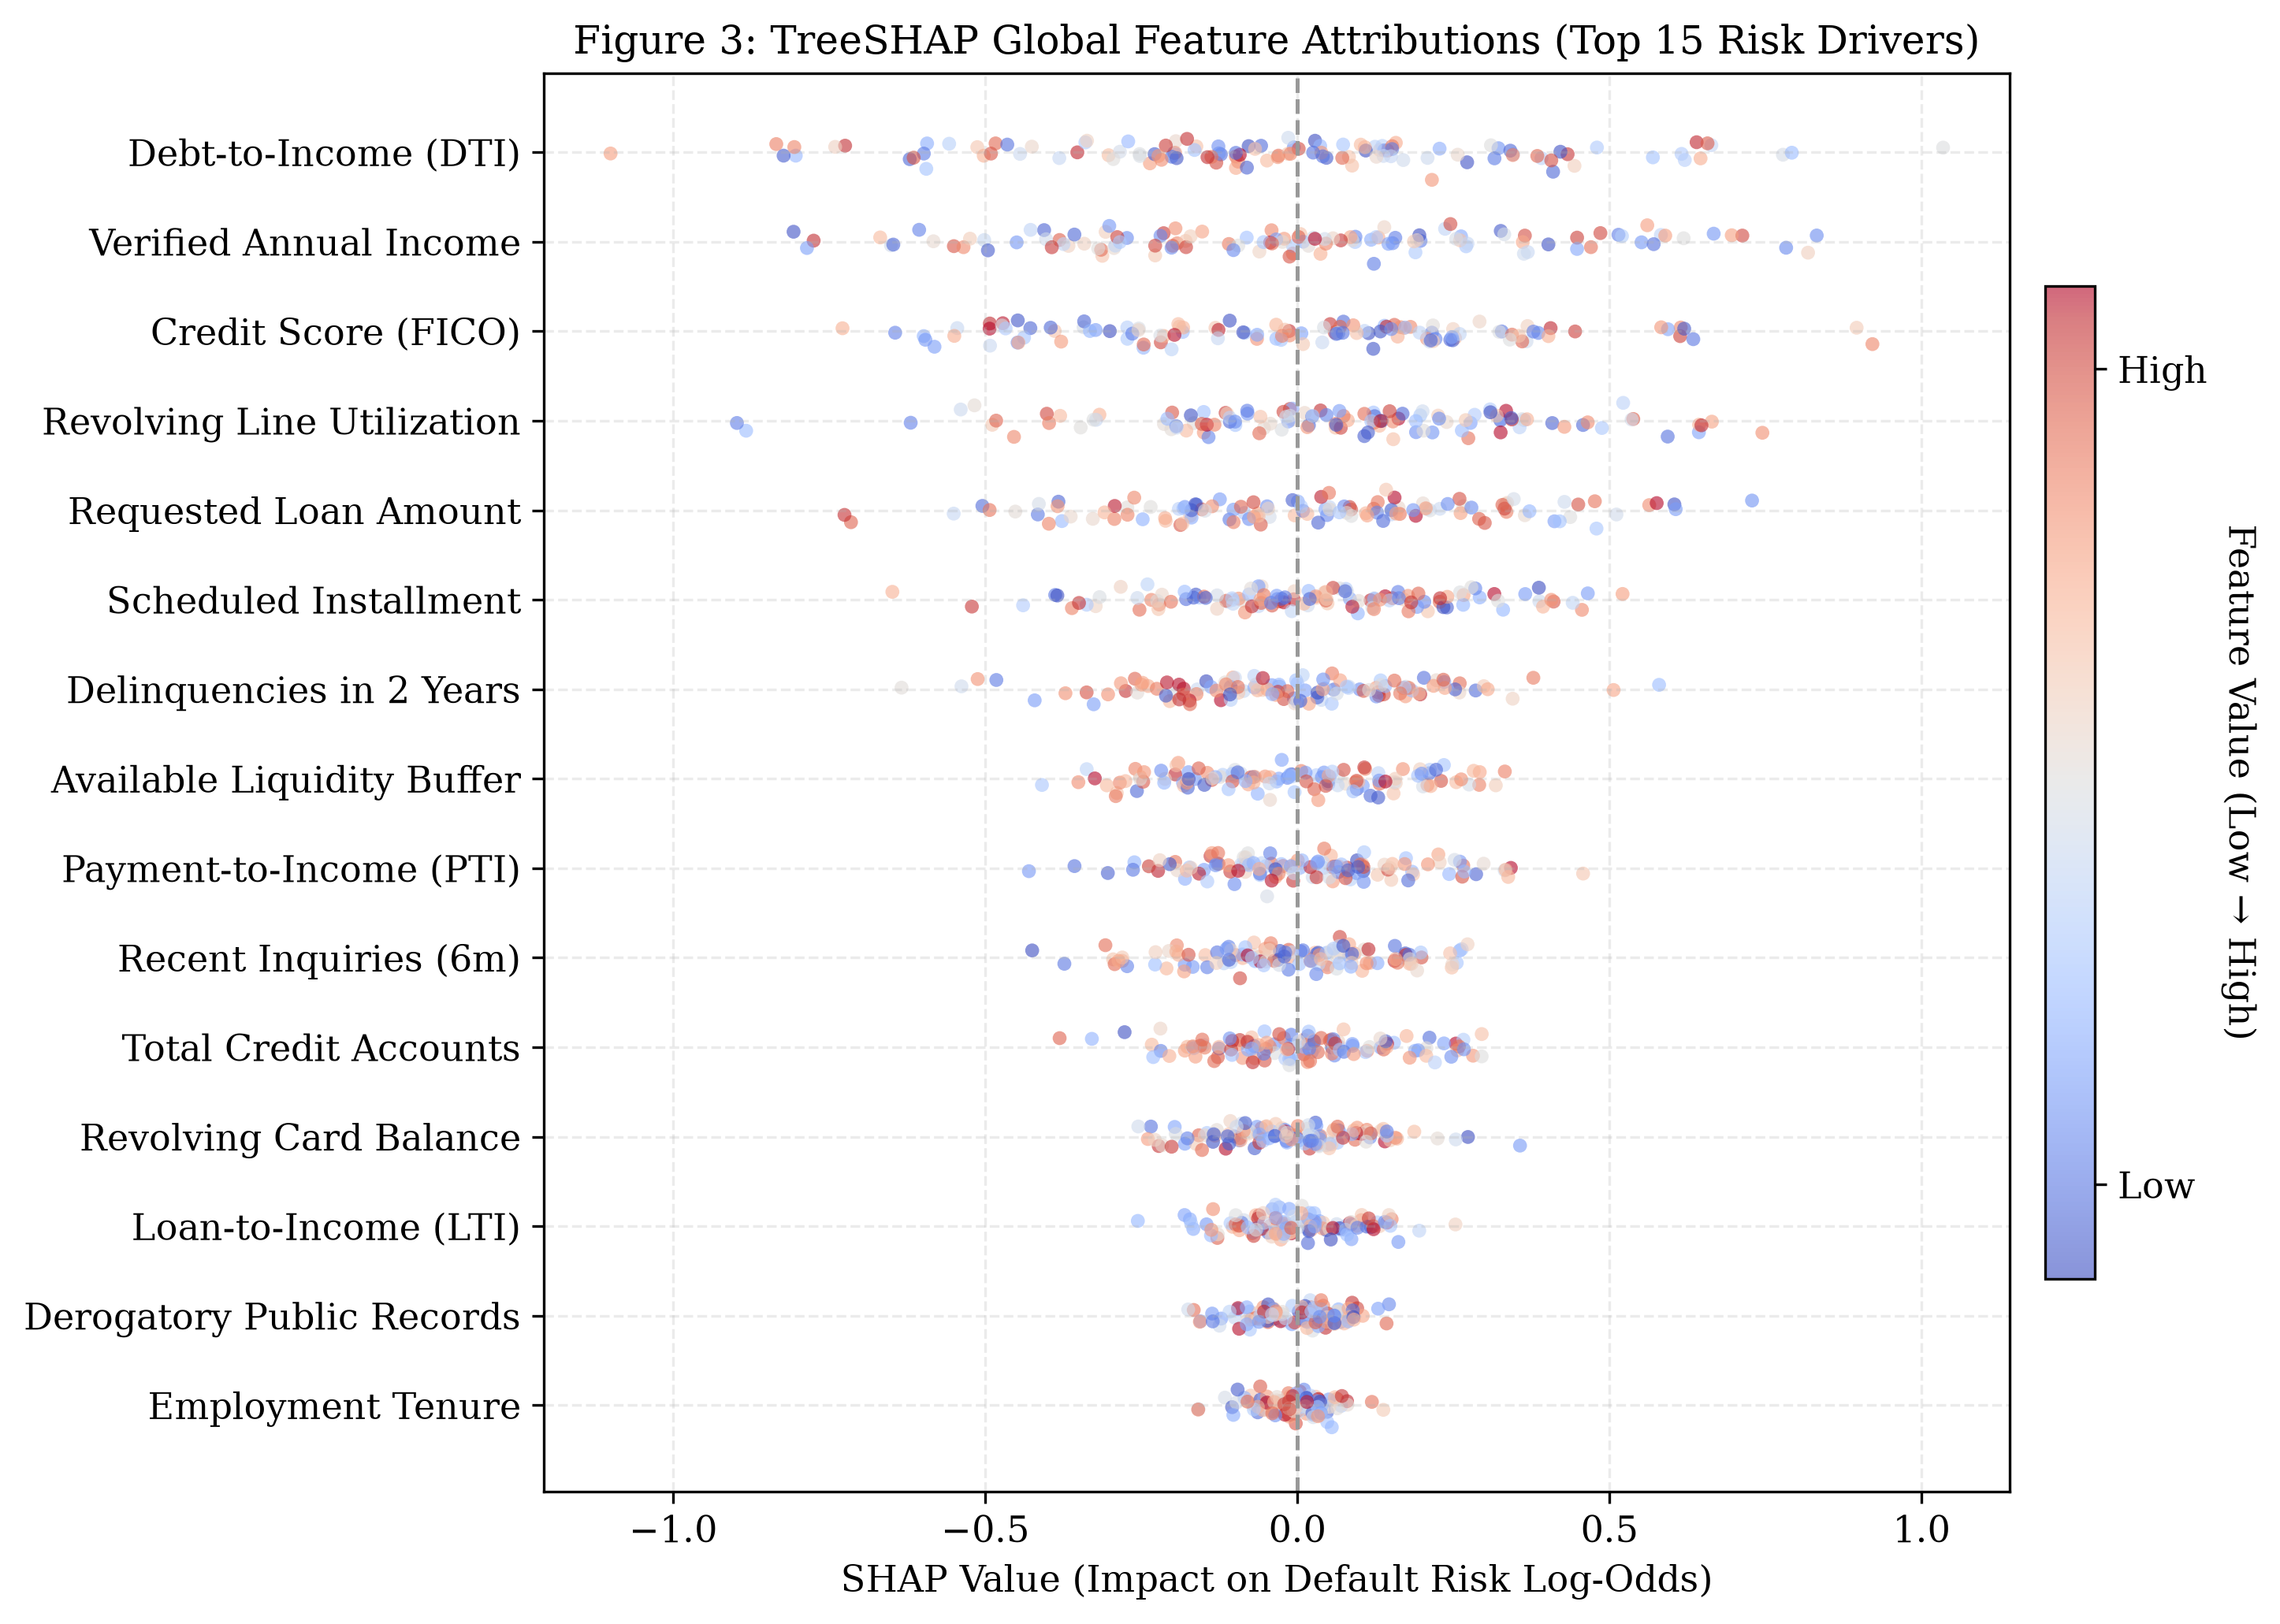
\includegraphics[width=\textwidth]{reports/paper/figures/fig3_shap_global_beeswarm.png}
        \caption{Global TreeSHAP Feature Attributions}
        \label{fig:shap_beeswarm}
    \end{subfigure}
    \hfill
    \begin{subfigure}[b]{0.49\textwidth}
        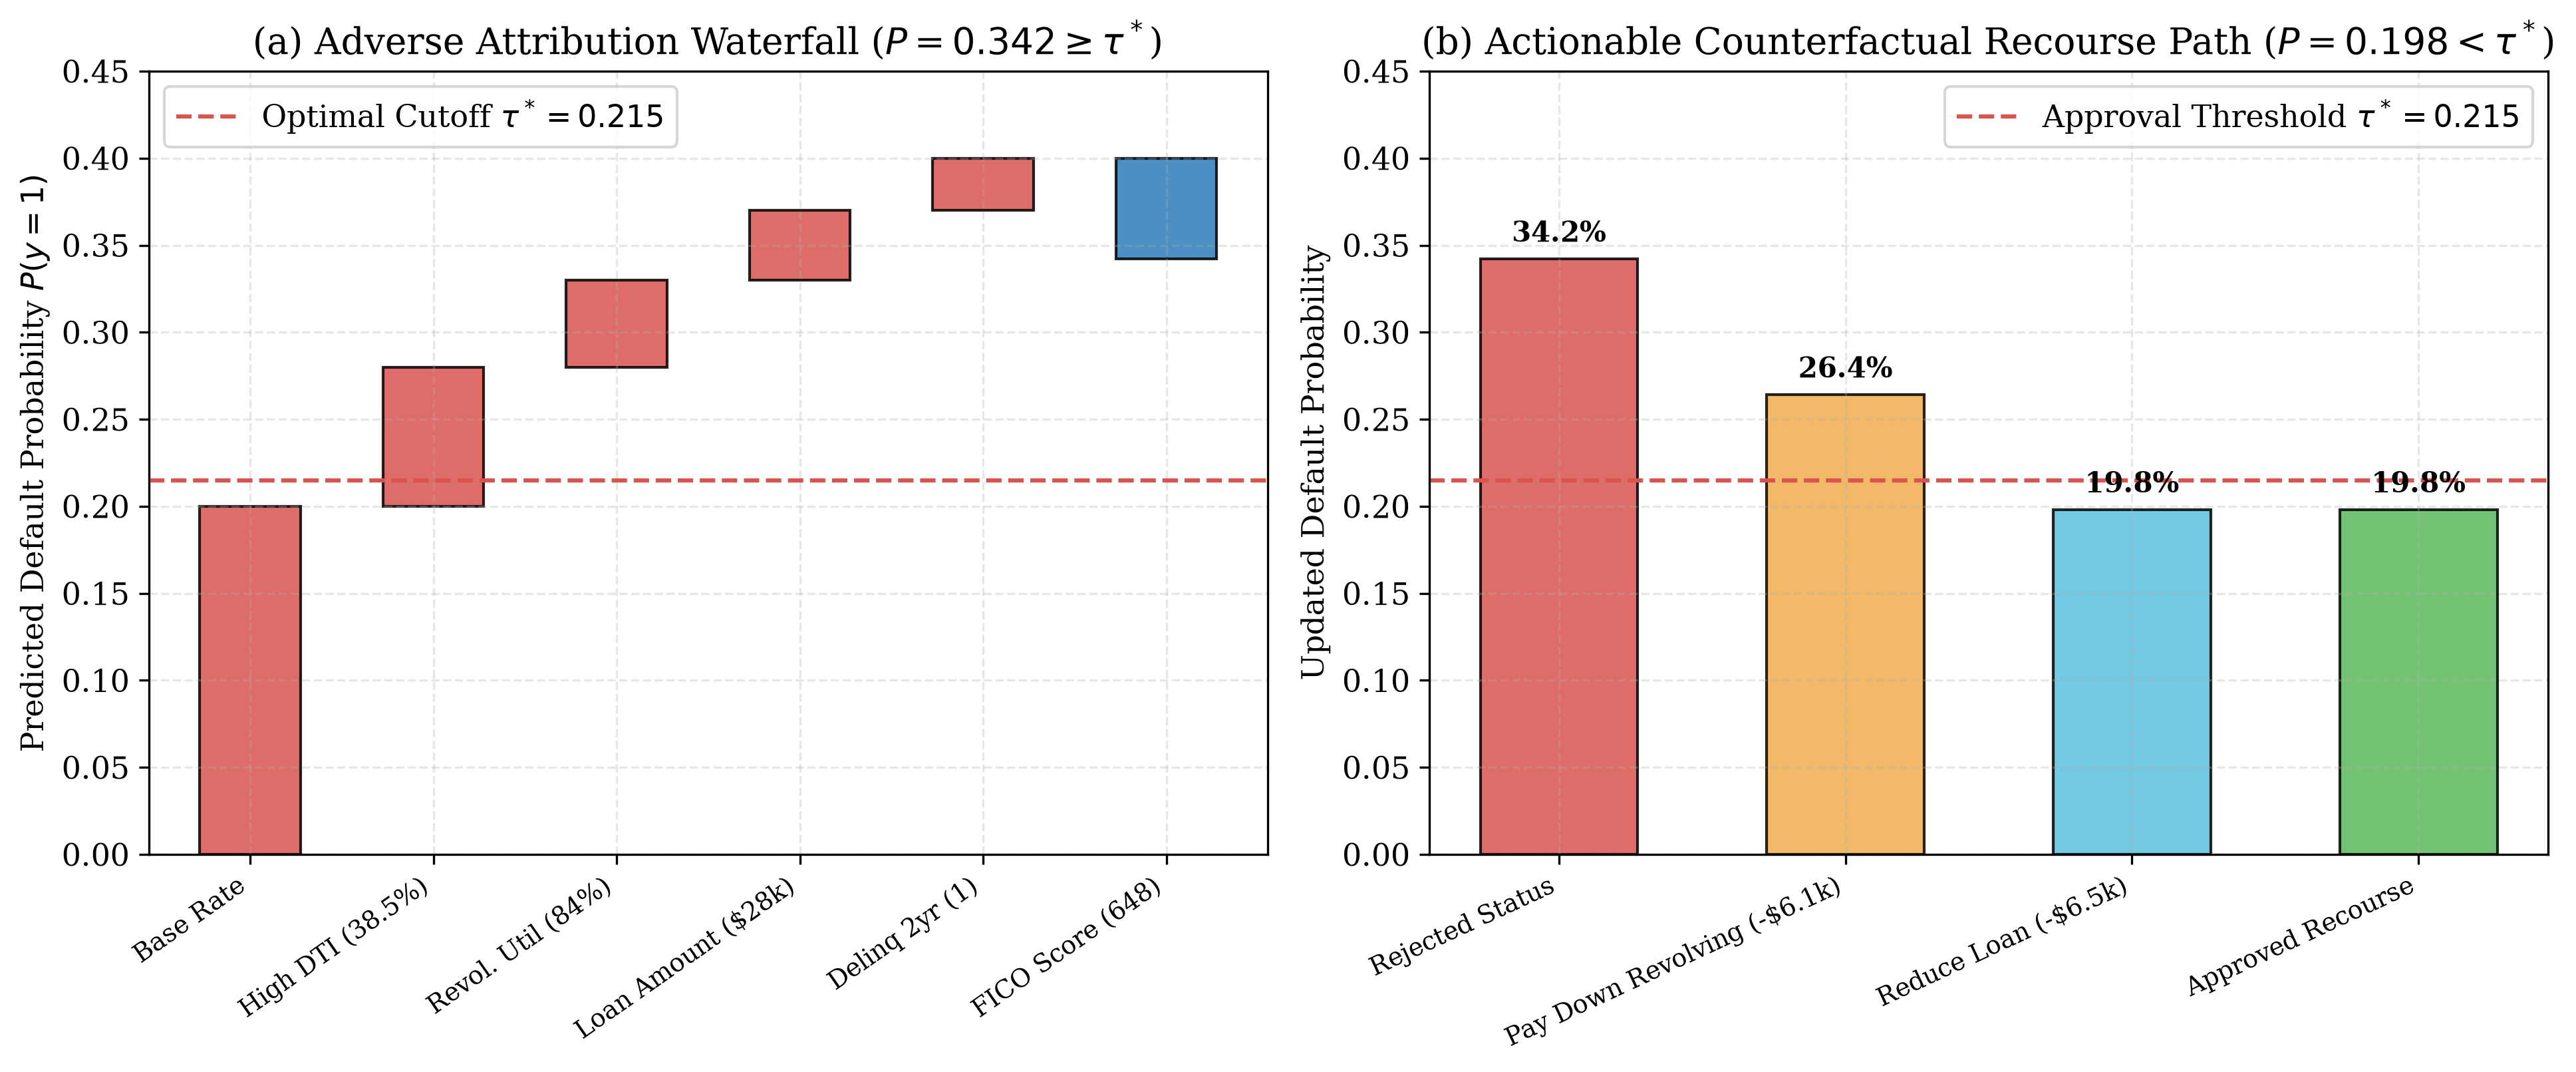
\includegraphics[width=\textwidth]{reports/paper/figures/fig4_actionable_recourse_waterfall.png}
        \caption{Adverse Action \& Recourse Path}
        \label{fig:recourse_waterfall}
    \end{subfigure}
    \caption{Interpretability and legally compliant actionable counterfactual recourse.}
    \label{fig:xai_recourse}
\end{figure}

Under the Equal Credit Opportunity Act (ECOA) Regulation B, lenders must deliver legally actionable explanations. Figure \ref{fig:xai_recourse} illustrates how Credex freezes immutable historical variables while solving for feasible financial recourse on mutable loan parameters.

\section{Conclusion}
This paper presented Credex, demonstrating that resolving the cost-symmetry fallacy via custom asymmetric gradients and threshold optimization yields dramatic balance sheet loss reductions (\$3.30M per 200,000 originations) while delivering compliant adverse action recourse.

\bibliographystyle{plainnat}
\begin{thebibliography}{99}
\bibitem[Elkan(2001)]{elkan2001foundations}
Elkan, C. (2001). The foundations of cost-sensitive learning. In \textit{International Joint Conference on Artificial Intelligence} (Vol. 17, No. 1, pp. 973--978).

\bibitem[Lessmann et al.(2015)]{lessmann2015benchmarking}
Lessmann, S., Baesens, B., Seow, H. V., \& Thomas, L. C. (2015). Benchmarking state-of-the-art classification algorithms for credit scoring: An update of research. \textit{European Journal of Operational Research}, 247(1), 124--136.

\bibitem[Li \& Wu(2024)]{li2024evaluating}
Li, Y., \& Wu, X. (2024). Evaluating machine learning models for credit scoring: A comprehensive empirical benchmark. \textit{Finance Research Letters}, 60, 104867.

\bibitem[Lundberg \& Lee(2017)]{lundberg2017unified}
Lundberg, S. M., \& Lee, S. I. (2017). A unified approach to interpreting model predictions. \textit{Advances in Neural Information Processing Systems}, 30, 4765--4774.

\bibitem[Xia et al.(2020)]{xia2020credit}
Xia, Y., Liu, C., Li, B., \& Liu, N. (2020). A boosted decision tree approach using Bayesian hyper-parameter optimization for credit scoring. \textit{Expert Systems with Applications}, 143, 113071.
\end{thebibliography}

\end{document}